%-----------------------------------------------------------------------------
%
%               Template for sigplanconf LaTeX Class
%
% Name:         sigplanconf-template.tex
%
% Purpose:      A template for sigplanconf.cls, which is a LaTeX 2e class
%               file for SIGPLAN conference proceedings.
%
% Guide:        Refer to "Author's Guide to the ACM SIGPLAN Class,"
%               sigplanconf-guide.pdf
%
% Author:       Paul C. Anagnostopoulos
%               Windfall Software
%               978 371-2316
%               paul@windfall.com
%
% Created:      15 February 2005
%
%-----------------------------------------------------------------------------


\documentclass[preprint]{sigplanconf}

% The following \documentclass options may be useful:

% preprint      Remove this option only once the paper is in final form.
% 10pt          To set in 10-point type instead of 9-point.
% 11pt          To set in 11-point type instead of 9-point.
% authoryear    To obtain author/year citation style instead of numeric.

\usepackage{amsmath}
\usepackage{graphicx}

\usepackage{color}
\usepackage{listings}
\lstset{ %
language=Java,                % choose the language of the code
basicstyle=\footnotesize,       % the size of the fonts that are used for the code
numbers=left,                   % where to put the line-numbers
numberstyle=\footnotesize,      % the size of the fonts that are used for the line-numbers
stepnumber=1,                   % the step between two line-numbers. If it is 1 each line will be numbered
numbersep=5pt,                  % how far the line-numbers are from the code
backgroundcolor=\color{white},  % choose the background color. You must add \usepackage{color}
showspaces=false,               % show spaces adding particular underscores
showstringspaces=false,         % underline spaces within strings
showtabs=false,                 % show tabs within strings adding particular underscores
frame=single,           % adds a frame around the code
tabsize=2,          % sets default tabsize to 2 spaces
captionpos=b,           % sets the caption-position to bottom
breaklines=true,        % sets automatic line breaking
breakatwhitespace=false,    % sets if automatic breaks should only happen at whitespace
escapeinside={\%*}{*)}          % if you want to add a comment within your code
}

\begin{document}

\special{papersize=8.5in,11in}
\setlength{\pdfpageheight}{\paperheight}
\setlength{\pdfpagewidth}{\paperwidth}

\conferenceinfo{CONF 'yy}{Month d--d, 20yy, City, ST, Country} 
\copyrightyear{2015} 
\copyrightdata{978-1-nnnn-nnnn-n/yy/mm} 
\doi{nnnnnnn.nnnnnnn}

% Uncomment one of the following two, if you are not going for the 
% traditional copyright transfer agreement.

%\exclusivelicense                % ACM gets exclusive license to publish, 
                                  % you retain copyright

%\permissiontopublish             % ACM gets nonexclusive license to publish
                                  % (paid open-access papers, 
                                  % short abstracts)

\title{Assisted Improvement of Software Documentation}

\authorinfo{Matthew Pearson-Beck \and Jeffrey Principe}
           {The University of Virginia}
           {\{mjp2ff, jwp3ce\}@virginia.edu}
           
\maketitle

\begin{abstract}
Software documentation helps developers understand code and aids in the process of maintaining software. However, documentation is frequently inconsistent and out-of-date, limiting its usefulness to developers, particularly in large projects where there is too much code to efficiently identify and fix poor documentation.

We propose an algorithm that helps developers identify poor documentation of Java methods and update it more efficiently and effectively. The algorithm searches for four key concepts in source code and compares them with the accompanying summary documentation. A ranked list of the worst-documented methods is presented to developers with suggestions for improvement.

We test our algorithm with a group of developers tasked with updating method documentation. Results show no correlation between use of the tool and an increase in overall speed or documentation quality, but provide insights into future work to reduce the quantity of suggestions and improve the human-readability of the algorithm's output.
\end{abstract}

% general terms are not compulsory anymore, 
% you may leave them out
\terms
documentation, human factors

\keywords
Javadoc, methods, machine learning, symbolic execution, natural language processing

\section{Introduction}
Maintenance is the most time-consuming part of the software development process, taking up two-thirds of development time \cite{buse10}. Documentation is a key component of software maintenance, helping developers understand code \cite{desouza}. However, most developers agree that software documentation is frequently incomplete or out-of-date, limiting its usefulness to developers \cite{lethbridge}. With many large projects containing over 1 million lines of code, searching for and updating poor documentation quickly becomes prohibitively expensive and time-consuming \citep{windows, mac, linux}.

This paper focuses on the documentation of procedures, particularly in large software projects. Functions and methods are the functional unit of many programming languages, making them an important unit to document. For the Java programming language, Javadoc provides a standardized way of documenting methods. Javadoc comments allow developers to specify application programming interface (API) documentation for methods for use by application programmers, quality control engineers and external groups making use of the application \cite{kramer}.

Though Javadoc provides a way to specify many types of information about methods, we restrict attention to the summary of the method's functionality, typically seen in the first sentence or two of the comment's general description. We propose an algorithm for the Assisted Improvement of Documentation (AID) which identifies concepts present in the source code that are missing in the accompanying summary description and presents a prioritized list of the worst-documented methods along with suggestions for developers to improve them.

AID seeks to reduce the time necessary to improve the documentation of methods in a large project and enable the creation of higher-quality documentation. A two-stage human study reveals a slight reduction in the difficulty of updating documentation when using AID's output. However, it does not find any correlation between the use of AID and a reduction in the time taken to write updated documentation or an improvement in the overall quality of the documentation.

This paper's main contributions are:
\begin{itemize}
\item A study of method summary descriptions in the Java programming language for well-documented methods of the Java Development Kit. Key concepts present in these methods leads to a model for summary documentation of Java methods in the general case.
\item An algorithm that identifies values for the key concepts that should be present in summary documentation and searches for them in documentation. Methods are prioritized on the overall difference between the concepts present in the source and those discussed in the comments.
\item A preliminary implementation of AID and an accompanying human study of its effectiveness in improving the efficiency and resulting quality of updating documentation with the use of AID. The results are inconclusive using the current prototype, but they provide a series of next steps for improving the effectiveness of AID.
\end{itemize}

\section{Motivating Examples}
Projects that are large in scope and develop over a long period of time often have documentation that does not reflect the current state of the code \cite{lethbridge}. These examples are not meant to criticize the projects in question, but merely to illustrate a problem that occurs through large software projects, and is realistically unavoidable as they grow and change over time.

Consider the method shown below, from the jEdit project, a text editor for programmers \cite{jedit}.

\begin{lstlisting}
/** Performs doMigrate() on each installed 
        OneTimeMigrationService */
public static void execute()
{
    String[] migrations = ServiceManager.getServiceNames(OneTimeMigrationService.class);
    if (migrations.length == 0) return;
    for (String migration: migrations)
    {
        Object obj = ServiceManager.getService(OneTimeMigrationService.class, migration);
        OneTimeMigrationService svc = (OneTimeMigrationService) obj;
        svc.doMigration();
    }
}
\end{lstlisting}

The comments associated with this method are inadequate for a few reasons. First, the methods actual purpose is discussed briefly and insufficiently, and it specifies the method call incorrectly. The comments do not discuss data or method flow, nor the purpose or details of the actions performed. Finally, the comments rely heavily on general class information to explain the method's purpose. This is problematic, because someone trying to use this method might be viewing the comments through Javadoc as they write code, rather than looking at the class' source directly.

Consider the second example, shown below. This method is from the TV-Browser project, a Java-based TV guide \cite{tvbrowser}.

\begin{lstlisting}
/**
   * reads an instance from a DataInput.
   *
   * @param in the input to read from
   * @return the new created instance
   * @throws IOException if somethin went wrong
   */
public static Date readData(final DataInput in) throws IOException
{
    int version = in.readInt();
    short year;
    byte month;
    byte day;
    if (version == 1) {
        // currently, version==3 is used
        int date = in.readInt();
        long l = (long) date * 24 * 60 * 60 * 1000;
        java.util.Date d = new java.util.Date(l);
        Calendar mCalendar = Calendar.getInstance();
        mCalendar.setTime(d);
        year = (short) mCalendar.get(Calendar.YEAR);
        month = (byte) (mCalendar.get(Calendar.MONTH) + 1);
        day = (byte) mCalendar.get(Calendar.DAY_OF_MONTH);
    }
    else if (version == 2)
    {
        year = (short) in.readInt();
        month = (byte) in.readInt();
        day = (byte) in.readInt();
    }
    else
    {
        year = in.readShort();
        month = in.readByte();
        day = in.readByte();
    }
    return new Date(year, month, day);
}
\end{lstlisting}

Again, the comments here have a few major flaws. The method's behavior is only described in a vague, general way that restates the method's name. There are spelling errors in the Javadoc header. There is no mention that the method's behavior is completely different based on the version of DataInput, an integral part of the method. Finally, there is no explanation of how each version is specifically handled.

\section{Exploration of Method Summary Documentation}
Though software documentation can reference many different types of information, certain concepts appear in the documentation for many methods. To that end, we sampled documentation from various methods from the Java Development Kit version 7 (JDK).

All of the methods in 11 JDK classes were sampled. With only a handful of exceptions, all of the public methods contained a Javadoc comment, and had at least one sentence in the general description section of the comment. Since the JDK provides descriptions for core libraries in the Java language, it establishes a documentation standard for other Java projects. Therefore, we believe that summary documentation in Javadoc comments is both prevalent and relevant in well-documented Java code.

The summary sentences of the methods analyzed contained many common structural and semantic components. Four concepts in particular were particularly common in summary descriptions. These were a verb describing the primary action undertaken by the method, a description of a primary object acted upon by the method, conditions that input parameters must satisfy for the method to execute normally, and other variables or objects that are important to the method's functionality.

For example, the \verb|equals()| method within the String class in the JDK provides the following description at the beginning of the method's Javadoc comment:

\begin{quotation}
Compares this string to the specified object. The result is true if and only if the argument is not null and is a String object that represents the same sequence of characters as this object.
\end{quotation}

In keeping with the typical documentation pattern of the JDK, \verb|equals()| begins its description by providing the action undertaken by the method (compares). This specific method has two primary objects, \verb|this| and the object passed to the method for comparison. Both are mentioned immediately after the primary action with ``this string to the specified object''. While there are no explicit exceptions thrown by the \verb|equals()| method, the conditions for reaching the normal execution path are described next, followed by an additional description of attributes of the relevant variables in the method's execution.

We use this analysis to focus on the four components of summary documentation described above. Our approach for identifying these concepts in source and comparing them to comments is described in the next section.

\section{Algorithm Description}
To address the issue of creating high-quality summary documentation for Java methods, we propose an algorithm that scans specified Java methods and their accompanying Javadoc descriptions, creating a ranked list of methods with suggestions for improving their documentation. In its simplest form, the algorithm accepts a single location of a directory, file, or Ant buildfile and scans all methods therein contained. More complex configurations allow for individual methods to be included in or excluded from analysis.

\begin{figure*}
	\begin{center}
		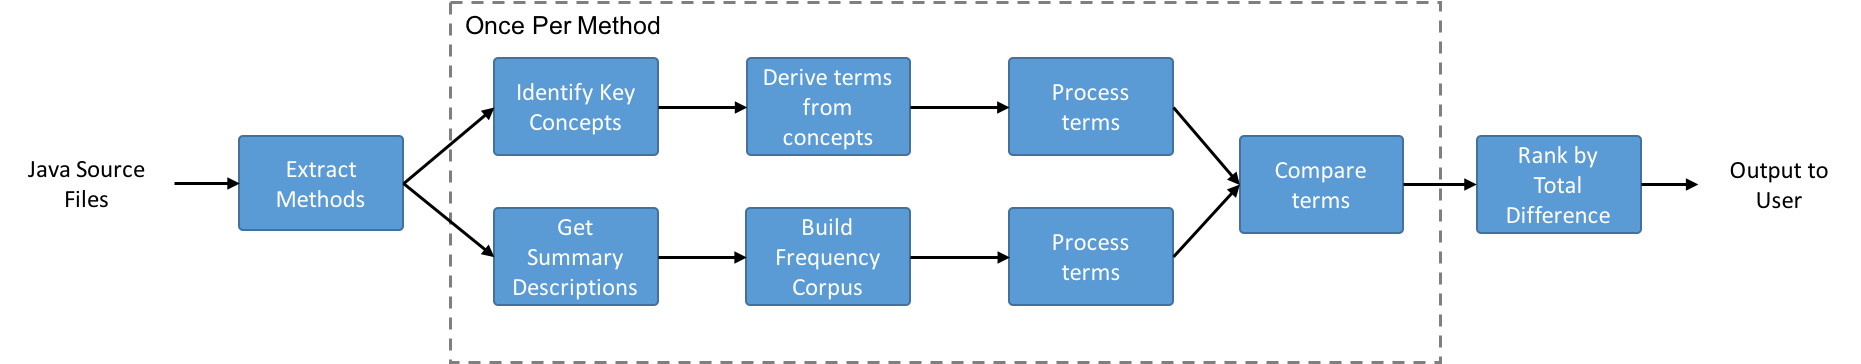
\includegraphics[width=\linewidth]{algorithm-structure.png}
	\end{center}
	\caption{High-level representation of the algorithm implemented in this paper. Once the methods are extracted from the source, the source code and comments are processed separately, yielding sets of terms from each that are compared, leading to an overall difference score. The methods are ranked by their scores and the worst are outputted to the user.}
	\label{figure-algorithm-summary}
\end{figure*}

The overarching algorithm used is fundamentally sequential in nature. A series of processing steps search for each of the four key concepts discussed above. These concepts are first identified in the method source and key terms are extracted from the content of each concept (section 4.1). Next, each term is processed and compared with the summary description of the method, receiving a relative significance of the difference if the term is not present (section 4.2). Finally, methods are sorted based on the values assigned to each missing term and those with the highest overall scores--those that are worst-documented--are presented to the user, along with suggestions for improving the documentation (section 4.3).

\subsection{Key Concept Identification}
Once a method has been found in the source code, several processing operations are performed to search for appropriate values for each of the four key concepts identified in the method summary documentation analysis (section 3). Each concept's analysis operates independently of one another and outputs a set of zero or more terms that should be present in the documentation.

\subsubsection{Primary Action}
Usually a one-word verb, the primary action summarizes all of the statements of the method. Since one verb must be derived from many statements or operations in the method's concept that may or may not make mention of the verb, standard program analysis techniques alone are a poor candidate for primary action identification. Instead, machine learning is used to synthesize a model for determining the higher level model from underlying parameters derived from standard program analysis techniques.

Machine learning presents its own challenges. Classification algorithms require a list of categories into which instances are grouped. The verb options for the primary action quickly become too numerous to be practical as categories in an n-way classifier. Rather than trying to enumerate as many verbs as possible, we selected a small set of common actions to classify. The verbs covered by these actions are compute, compare, convert, create, get, set and test.

However, this seven-way classifier is incomplete, since some methods do not belong to any of the above categories. For those methods, another category was added to the classifier, indicating that a fallback should be used to determine the primary action. The method's name serves as a reasonable fallback, since Java naming conventions often lead to method names that contain a verb describing the action of the method. Though this fallback relies on the original developer writing a descriptive method name, it provides some information for methods that could not otherwise be classified.

\begin{table}
	\begin{center}
		\begin{tabular}{ l | c | c | c | c | c }
		Category & TP Rate & FP Rate & Precision & Recall & F1-meas. \\
		\hline
		compute & 0.407 & 0.027 & 0.55 & 0.407 & 0.468 \\
		compare & 0.182 & 0 & 1 & 0.182 & 0.308 \\
		convert & 0 & 0.003 & 0 & 0 & 0 \\
		create & 0.807 & 0.016 & 0.902 & 0.807 & 0.852 \\
		get & 0.89 & 0.443 & 0.337 & 0.89 & 0.489 \\
		set & 0.091 & 0.046 & 0.167 & 0.091 & 0.118 \\
		test & 0.64 & 0.05 & 0.485 & 0.64 & 0.552 \\
		\emph{fallback} & 0.209 & 0.083 & 0.523 & 0.209 & 0.299
		\end{tabular}
	\end{center}
	\caption{Classifier results for each of the categories classified. Create, test and get perform the best, while set and convert perform the worst.}
	\label{table-classifier}
\end{table}

The final seven-way Naive Bayes classifier was populated with a training set of 362 methods pulled from several files in the Java Development Kit, version 7. When tested in 10-fold cross-validation, 45.9\% of methods were correctly classified, compared with 48.3\% when testing directly on the training data set. Notable strengths include the create, test and get categories, with F1-measures of 0.852, 0.552 and 0.489 under cross-validation. Overall, the classifier performs with an F1-measure of 0.417, compared with 0.141 for the best-case trivial categorization of all methods into the fallback category. Therefore, we assert that this model does a significantly better job of identifying the primary action than simply using the method name for everything, particularly when the original developer is not trusted to include the primary action in the method name.

Once a category has been assigned to the method's primary action, the primary action is recorded in a single term for detection in the method's comments; this comparison is discussed in Section 4.3 below. The term used for the six specific actions classified is the same as the verb used for the category label (e.g. convert). When using the fallback of the method name, the term used is the method's actual name (e.g. addObject for a method with name addObject).

\subsubsection{Primary Object}
The primary object represents the single most important identifier contained in the method, and is intended to represent the main object upon which the method acts or is otherwise most relevant to this method. This is an important aspect to the method's meaning, and should be featured in the method's comments in order to properly address the method's behavior.

In order to identify the primary object in a method, we analyzed a control flow graph of the method in order to determine which objects were acted upon in the way most relevant to the method's meaning. We relied on a control flow graph implementation from Anders Hessellund \cite{hessellund}.

There were two main approaches to analyzing the control flow graph. The first focused on the paths upon which an identifier appeared; we found the identifier that appeared on the most paths leading to a successful function exit (either return statement or otherwise, but not an exception). This was our default process and was used in most cases. However, due to the control flow graph implementation as well as ties between multiple identifiers, there were cases in which this process failed.

In the case of the first process failing, our fallback approach focused on the statements upon which an identifier appeared; we found the identifier that appeared on the most statements on any path to a successful function exit. This was more rudimentary than the first process, but worked more generally when the first failed.

\subsubsection{Conditions for Success}
Though determining exceptional behavior in is undecidable in the general case, a reasonable approximation can be made through static analyses. Previous efforts have been made to specifically address documenting exceptions, which is largely accomplished through symbolic execution \cite{buse08}. A similar approach is employed here.

In this intraprocedural analysis, we focus on explicit throws statements contained within a method and the predicate that must be satisfied for each statement to be reached. Once all of the throws statements are found in a method, paths to each statement are enumerated using a control flow graph generated from an off-the-shelf tool. Loop bodies are treated like if statements, executing either 0 or 1 times depending on the path. While such a simplification can lead to incorrect judgments upon evaluation, it allows for reasonably accurate determinations to be made in many cases.

Next, each path to a throws statement is symbolically executed. Each parameter and field used in the method is set to a placeholder initial value, and each statement with an assignment updates the value of the variable on the left side of the assignment. When a predicate such as an if statement condition is encountered, the expression is evaluated using symbolic values for the relevant variables at that point in execution. All of the predicates for a given path are combined via conjunction. To determine the predicate necessary to avoid all of the throws statements, the predicates for all exceptional paths are combined with disjunction, then negated.

At this point, the conditions for success are mathematically complete. However, many duplicate predicates exist due to the same conditions being executed along many paths. To make the predicates more compact and easier for humans to understand, several simplification steps are performed. First, constant algebraic expressions are evaluated. Then, trivially satisfiable and unsatisfiable sub-predicates are identified and redundant conditions that are either equal to or subsumed by another predicate are removed.

The resulting predicate is converted into a human-readable form by replacing different expression types with a human-readable representation of the expression. Due to the nature of the manipulations performed, the resulting predicate often takes the form of a list of predicates joined by conjunction. To improve readability and granularity of comparison, each term in the conjunction is treated separately. The terms present in the human-readable form of each predicate are used for comparison with the comments. Methods with no throws statements return an empty term list and are ignored during comparison (Section 4.3).

\subsubsection{Additional Components}
Unlike the other three key concepts identified in method source, additional components can include many different items. For the purposes of this analysis, we chose to focus on the use of parameters and fields in the method, as well as information derived from the method's name.

Relative importance of individual variables is determined using the density of reads and writes involving that variable. Each statement is analyzed for uses of variables. If a variable is present on the left hand side of an assignment, a write is logged. Any other use of a variable (including method invocations) is logged as a read. Each parameter or field used at least once is logged as a term for comparison. The number of reads and writes for each is used later to help determine the relative importance of any inconsistencies.

\subsection{Comment Processing}
We integrated two natural language processing (NLP) techniques to process the comments we read from the program text in order to standardize them without losing any meaning. Specifically, we focused on processing human-written sentences prior to comparison between comments and the code they are associated with. These techniques are discussed below.

\subsubsection{Word Stemming}
Word stemming is the process of converting inflected or derived words to their most basic form \cite{xapian}. This allows us to recognize, for example, that ``run'' and ``running'' are forms of the same word. We used the Snowball Stemmer \cite{snowball} to process all the text read in from comments associated with each method, and saved the processed results for future comparison.

\subsubsection{Stoplisting}
Stoplisting is the process of removing selected words that are deemed unimportant or insignificant to the overall meaning of natural language \cite{rajaraman}. Some examples of words we would stoplist are ``the'' and ``is''. Whether these words appear in both, either, or neither of the code or associated comments is unimportant. For our algorithm, we took our stemmed words and removed any that were present in an extensive list of commonly stoplisted words \cite{xpo6}.

\subsection{Comparison and Ranking}
After analyzing the code for a method and processing the associated comments, the last step in our algorithm is to compare the two and provide a measurement for how effective the documentation is. We use two specific techniques discussed below to modify the comparison, but beyond that we simply do a set comparison.
This comparison is between the expected words determined from the analyzed code and the processed words found in the comments. Any word we determined important that was not featured in the comments is a penalty against that method's comments, in the form of a ``difference score'' given to each method. The lower the difference score, the better the method's comments.

\begin{table}
	\begin{center}
		\begin{tabular}{ l | c }
		Concept & Maximum Penalty \\
		\hline
		Primary Action & 25 \\
		Primary Object & 25 \\
		Conditions for Success & 15 \\
		Additional Components & 25 \\
		\end{tabular}
	\end{center}
	\caption{Maximum penalty that can be assessed to a method's documentation for each major concept. If there are multiple penalties assessed under a single major concept (common for additional components), their sum will not exceed the maximum weight shown here. Conditions for success receives a smaller maximum penalty than the others because it appears less often in code that is considered well-documented.}
	\label{table-concept-penalty}
\end{table}

For each difference score, there are a few set penalties that are applied based on the code analysis done above. Each concept receives a maximum difference score that can be associated with it. Within the additional components group, any penalty is distributed proportionally among the constituent variables, which are separately weighted based on the number of reads and writes as well as whether each is a field or parameter. Table \ref{table-concept-penalty} shows the weights applied to each major concept, and the relative contribution of uses to a variable's share of the additional components penalty.

\subsubsection{TF/IDF}
TF/IDF is a statistical analysis that identifies the relative importance of a specific word as a part of a larger body, or corpus, of words \cite{stanford}. A term is considered more important if it appears many times in the current document, as well as if it appears in relatively few documents compared to the size of the corpus.

We use this as part of our text analysis to give each word relatively more or less significance based on its use, and more impact on the difference score. This is capped at a maximum value for each term, so that no one word, no matter how important, cannot individually invalidate a method's documentation. For our algorithm, the corpus was all the methods contained in the project to be analyzed, and each method is treated as an individual document.

TF/IDF is integral to our comment analysis and comparison, because a word that appears throughout the corpus is likely not relevant to this specific method, and does not need to appear in the documentation.

\subsubsection{WordNet}
WordNet is a lexical database for the English language that is used to identify synonyms \cite{wordnet}. We used the WordNet library to recognize when two different words represented the same concept.

In comparing terms from the analyzed methods and processed words from the associated comments, we performed a WordNet comparison to determine if the words were related, instead, instead of simply checking string equality. This allowed us to further recognize when the comments addressed the necessary information in an equivalent but differently-worded form.

\section{Evaluation}
Documentation must effectively describe its associated code for it to be useful. There is a tendency for documentation to fall out of date over time, especially in large projects \cite{forward}. As a result, maintaining good documentation becomes a serious problem beyond maintaining code itself.

We have implemented the algorithm described in Section 4 in the form of AID, a prototype tool that analyzes Java projects and highlights the method it determines have the most inadequate documentation. In this section we discuss our evaluation methodology as well as quantitative and qualitative results from a study of AID.

\subsection{Methodology}
We performed our evaluation with a two-part human study, conducted through the use of paid participants on Amazon's Mechanical Turk \cite{mturk}. All participants had to pass a basic Java competency quiz to ensure they were qualified for the task.

In the first part of our study, test subjects were given code for a method with the comments removed, along with relevant information from the surrounding class (class name, fields). Participants had to write comments that would go along with the highlighted method. Half the participants were given the output of AID to use in writing documentation, while the other half were not. Each participant completed this process for 10 methods. We had 100 participants complete the first part of the  survey, and we accepted 49 responses after removing those that did not follow the instructions or did not express an adequate understanding the given task. There were 20 total methods analyzed across all participants.

In the second part of our study, participants were given the code for a method with the comments removed, along with the same surrounding class information. They were then presented with 10 pairs of proposed comments for that method. The sample methods were taken from the result of the first part of the human study. Each pair contained one sample that was written with AID's results available and one without. Participants in the second part of the study selected which documentation sample they preferred in each pair, with the options being 1 (significantly prefer the left sample), 2 (slightly prefer the left sample), 3 (slightly prefer the right sample), and 4 (significantly prefer the right sample). The positions in which the documentation was presented, with respect to whether or not it used AID's results, was scrambled to avoid biases. Participants completed 10 pairs of documentation for each method, and completed 10 methods in total. The same 20 methods were analyzed here as in the first part of the study. Participants were also asked to describe qualities of good documentation at the end of the survey, which was used as a flag to show if they followed the instructions and understood the given task. We had 100 new participants complete the second part of the survey, and we accepted 45 responses after removing some based on the freeform question mentioned previously.

\subsection{Quantitative Analysis}
Overall effectiveness of AID is measured along three different metrics: difficulty, efficiency and quality of documentation. The first two metrics are derived from the first stage of the survey, while the third comes from the results of the second stage.

\subsubsection{Difficulty}
In the first stage of the human study, participants were asked to provide an assessment of the overall difficulty of updating documentation for the 10 methods they were presented with. Judgments were made on a Likert scale from 1-5, where 1 was very easy and 5 was very hard. Participants who were given use of the output from AID reported an average difficulty of 3.5, compared with 3.815 for those who did not have any assistance. A two-sample unequal variances t-test revealed that the result is significant at \(p = 0.0758\).

\subsubsection{Time to Document}
The time taken to write each piece of documentation in the first stage was recorded for comparison. Participants with access to the output of AID took 3:17 on average, while those without the tool took 3:15. However, a two-sample unequal variances t-test does not find the result significant, leading us to conclude that participants took equal time regardless of whether or not they were in the treatment group.

\subsubsection{Documentation Quality}
Most importantly, developers should be able to write better documentation with the use of AID. This was measured using judgments provided by participants in the second stage of the study. Results are first normalized such that higher values for the Likert rating always indicate a stronger preference for documentation generated with use of AID, with 4 indicating the strongest preference for AID-assisted documentation and 1 indicating the strongest preference against it. Once normalized, the average Likert rating is 2.487, with 2.5 indicating no overall preference. A one-sample t-test does not find a significant difference between the results and the expected mean; therefore, we cannot conclude any preference for or against documentation generated with the assistance of AID.

\subsection{Conditions for Success}
While respondents in stage two of the survey indicated no overall preference for or against documentation generated with the help of AID, this result does not necessarily apply to the individual concepts emphasized by the algorithm. In particular, we noticed that respondents emphasized the value of documentation that explains conditions for successful execution (see Section \ref{Qualitative Analysis}).

To determine the favorability of documenting conditions for success, we manually annotated each documentation instance from stage one of the study with whether or not it mentions the conditions for success for its associated method. Next, we restricted attention to only the pairings of documentation samples where one sample discusses conditions for success and the other does not. The resulting data set contains \(1581\) comparison of documentation samples.

\begin{figure}
	\begin{center}
	\end{center}
	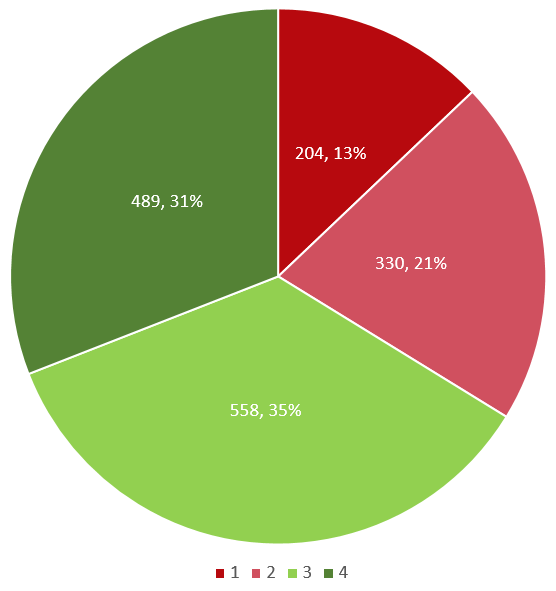
\includegraphics[width=\columnwidth]{conditions-for-success-likert.png}
	\caption{Favorability of documentation samples describing conditions for success. In \(1581\) comparisons between one documentation sample that describes conditions for success and one that doesn't, respondents indicated a preference for the sample that discusses conditions for success over \(66\%\) of the time, including over \(30\%\) who indicated a strong preference (Likert rating of \(4\)).}
	\label{figure-cfs}
\end{figure}

When comparing instances with documented conditions for success to those without, respondents provided an average Likert rating of \(2.842\), where \(4\) indicates a strong preference for documentation with conditions for success and \(1\) indicates a strong preference for documentation that does not mention success conditions. Using a one-sample t-test comparing against an expected average of \(2.5\), \(t = 13.55\) with \(1580\) degrees of freedom, yielding a significant result for \(p = 0.0005\). Overall, users indicated a preference for samples containing a description of conditions for success over \(66\%\) of the time and a strong preference over \(30\%\) of the time.

Since documentation writers given the output of AID were told specifically about the conditions for success, it stands to reason that they would document such conditions more often than those with no information. However, at a rate of \(41.4\%\), those with the use of AID only documented conditions for success slightly more often than those without it (\(40.8\%\)). One possible explanation is that AID either exposed too much information to documentation writers, making it tough to identify individual concepts that were important, or it did not make the information clear enough to understand. Another possibility is that a portion of developers do not believe conditions for success should be included in method summary documentation and chose not to include it even with the suggestion.

\subsection{Qualitative Analysis}
From our human studies, we gathered significant freeform feedback from our testers as to what they thought about the tool, how difficult it was to write documentation, what they valued in good documentation, etc.

Feedback about what constitutes good documentation repeatedly highlighted the importance of conciseness in documentation - shorter documentation that conveys the same information is more useful and desired. Comments in response to the prompt: ``Based on the documentation samples you read, identify a few characteristics of good documentation.'' included the following:

\begin{itemize}
\item ``Quick and concise.''
\item ``Good documentation is succinct.''
\item ``Complete and details in brief.''
\item ``Concise''
\item ``Not too long''
\end{itemize}

However, we found that documentation written by testers using AID was actually 10\% longer, on average, than documentation written without it. This suggests that users relied on AID and felt compelled to include all the information presented, rather than using it as a resource as intended. Further work needs to be put into improving the quality of output to inform users as to its intended purpose.

Users also valued the conditions for success identified by AID. In response to the same prompt, users said:

\begin{itemize}
\item ``The condition and if/else clauses are clearly mentioned''
\item ``...any error conditions...''
\item ``Under which conditions the method or class will throw an exception''
\end{itemize}

None of these users were exposed to the results of AID, so they could not know that we provided these conditions for success in our feedback. This suggests to us that these conditions for success should be more heavily incorporated into AID's responses, and presented more clearly to the user.

Finally, users also valued the primary action we identified through AID that concisely summarized the purpose of the method. Again, these users were not exposed to AID so did not know what it provided (nor even that it existed). Comments to this effect in response to the same prompt include:

\begin{itemize}
\item ``It should clearly state what the method does''
\item ``It should explain...what it is trying to accomplish.... It shouldn't list every variable and every single thing it does''
\item ``Correctly describe what it does''
\end{itemize}

This again suggests that AID should emphasize this feature, and make it more presentable so that users know how and when to make use of it in creating documentation.

\subsection{Threats to Validity}
There are a few major limitations to our human studies that may have affected the results. Firstly, we had fewer samples for the half (10/20) of our methods with the use of AID in the first part of our human study. This is because of the rate at which Mechanical Turk participants started the study and the distribution mechanisms for serving up methods. However, we believe that there are still enough samples for each method to ensure statistical significance in our results, although some configurations of method number and use/absence of AID have more samples than others.

Secondly, the order of methods served up in the first part of the human study was not randomized, so many people completed the same methods in the same order, which may have introduced unintended patterns of interaction or biases introduced by earlier methods on later ones. We have no way of measuring the effect of this, but we did mitigate this in the second human study by randomizing not only the order of methods shown, but the order of pairs shown within a method.

Finally, we measured the elapsed time that each user spent on each page in both parts of our human study, but we cannot guarantee that this is equivalent to the amount of time the user spent analyzing that method. They may have left their computer for a period of time, which could increase their elapsed time for one or many methods. There is no effective way to mitigate this. We attempted to look for anomalies in the elapsed time field for any one method for a specific user, but we were unable to determine with certainty any specific instances of this.

\section{Future Work}
There are many opportunities for further exploration in this field; our algorithm and implementation in the form of AID are just first steps in this area. A likely next step continuing from our implementation and using the results of the human studies would be to focus on reducing the length of the output from AID. Making it focus more on essential that components which are missing rather than providing breadth in its advice could lead to more concise and effective documentation.

One aspect that AID lacks is the ability to provide context for concepts that are missing in the method's comments. For example, giving context to the variable uses that are being considered in the code/comment comparison would make it easier for users to incorporate the most important aspects of the method into their documentation, moreso than simply knowing the names of the variables that are used.

AID's output itself provides a lot of information, but is not currently in the most human-readable format. Further study into the aesthetics and HCI for AID's output could provide good returns in overall documentation improvement. Not much focus was spent on this in the first iteration, in favor of algorithmic improvements.

At a more complex level, an area requiring significant further exploration is a study of AID's ability to identify the worst-documented methods in a project. We believe that AID can effectively identify poorly-documented methods, but we have not yet confirmed this with any kind of human study. If AID is effective in simply identifying the most poorly-documented methods out of a large group, this would provide a huge improvement in productivity by maximizing the benefit of time spent improving documentation project-wide.

\section{Conclusion}
Software maintenance is a costly and time-consuming portion of the software lifecycle. Documentation is a common resource used to assist developers with the process of maintaining software. However, software documentation is frequently inconsistent or out-of-date, reducing its usefulness. Documentation of methods can include many pieces of information, but almost always involves a high-level summary of the method's documentation.

We propose AID to help developers identify and improve poorly documented methods. The algorithm identifies four key concepts in a method's source code and tries to match them to descriptions in the accompanying documentation. Concepts missing in documentation contribute to a measure of the documentation's quality, which is then used to rank methods in order such that those that need the most attention are shown first. This ranked list of methods is shown to developers along with specific suggestions for improving poorly documented methods.

In a two-stage study of 49 and 45 Java developers, respectively, documentation was updated with slightly greater ease when developers were given the use of AID to assist them. Otherwise, developers produced documentation of roughly equal quality with or without the use of AID and did so in about the same amount of time. It is hypothesized that an increase in the length of documentation resulting from the use of AID contributed to this result. Further investigation is proposed in two areas: (1) reducing AID's output to essential components of documentation that are missing and (2) transforming the output into a more human-friendly form.

\acks

Acknowledgments, if needed.

% We recommend abbrvnat bibliography style.

\bibliographystyle{abbrvnat}

% The bibliography should be embedded for final submission.

\begin{thebibliography}{}
\softraggedright

\bibitem{jedit}
http://www.jedit.org/

\bibitem{tvbrowser}
http://www.tvbrowser.org/

\bibitem{hessellund}
https://www.itu.dk/people/sestoft/papers/hessellund-sestoft-ecoop.pdf

\bibitem{snowball}
http://snowball.tartarus.org/

\bibitem{xapian}
http://xapian.org/docs/stemming.html

\bibitem{rajaraman}
http://i.stanford.edu/~ullman/mmds/ch1.pdf

\bibitem{xpo6}
http://xpo6.com/list-of-english-stop-words/

\bibitem{stanford}
http://nlp.stanford.edu/IR-book/html/htmledition/tf-idf-weighting-1.html

\bibitem{wordnet}
https://wordnet.princeton.edu/

\bibitem{mturk}
https://www.mturk.com/mturk/welcome

\bibitem{buse08}
https://www.cs.virginia.edu/~weimer/p/weimer-issta2008-docinf.pdf

\bibitem{buse10}
https://www.cs.virginia.edu/~weimer/p/weimer-ase2010-deltadoc-preprint.pdf

\bibitem{windows}
https://www.facebook.com/windows/posts/155741344475532

\bibitem{mac}
http://www.engadget.com/2006/08/07/live-from-wwdc-2006-steve-jobs-keynote/

\bibitem{linux}
https://web.archive.org/web/20131219054847/http://www.h-online.com/open/features/What-s-new-in-Linux-3-6-1714690.html?page=3

\bibitem{desouza}
de Souza, S. C. B., Anquetil, N., \& de Oliveira, K. M. (2005). A study of the documentation essential to software maintenance. In Proceedings of the 23rd annual international conference on Design of communication: documenting \& designing for pervasive information (pp. 68-75). doi:10.1145/1085313.1085331

\bibitem{lethbridge}
Lethbridge, T. C., Singer, J., \& Forward, A. (2003). How software engineers use documentation: The state of the practice. Software, IEEE, 20(6), 35-39. doi:10.1109/MS.2003.1241364

\bibitem{kramer}
Kramer, D. (1999). API documentation from source code comments: a case study of Javadoc. In Proceedings of the 17th annual international conference on Computer documentation (pp. 147-153). doi:10.1145/318372.318577

\bibitem{forward}
Forward, A., \& Lethbridge, T. C. (2002). The relevance of software documentation, tools and technologies: a survey. In Proceedings of the 2002 ACM symposium on Document engineering (pp. 26-33). doi:10.1145/585058.585065

\end{thebibliography}


\end{document}

%                       Revision History
%                       -------- -------
%  Date         Person  Ver.    Change
%  ----         ------  ----    ------

%  2013.06.29   TU      0.1--4  comments on permission/copyright notices

